% TdeGPAE es el archivo principal para construir el Tarbajo de Grado en Estad\'{\i}stica en la Universidad del Valle

% EncabezadoPAE carga los paquete necesarios para ejecutar TdeGPAE

\documentclass[12pt,spanish,fleqn,openany,letterpaper,pagesize]{scrbook}


% Esta plantilla utiliza un formato de codificaci\'{o}n est\'{a}ndar
% Cada usuario puede utilizar las instrucciones adecuadas para su propio sistema operativo
\usepackage[latin1]{inputenc}

\usepackage{graphicx}
\usepackage{colortbl}
\usepackage{multirow, array} % para las tablas
\usepackage{float} % para usar [H]
\usepackage{color}
\usepackage{soul}
\usepackage[spanish]{babel}
\usepackage{fancyhdr}
\usepackage{graphicx,epsfig}
\usepackage{amsmath}
\usepackage{amssymb}
\usepackage{natbib}
\usepackage{tabularx}
\usepackage{longtable}
\usepackage{hyperref}
\usepackage{url}

\usepackage[none]{hyphenat}
    \sloppy

\usepackage{ragged2e}
	\justifying

\renewcommand{\theequation}{\thechapter-\arabic{equation}}
\renewcommand{\thefigure}{\textbf{\thechapter-\arabic{figure}}}
\renewcommand{\thetable}{\textbf{\thechapter-\arabic{table}}}

\pagestyle{fancyplain}
\textheight22.5cm
\topmargin0cm
\textwidth16.5cm
\oddsidemargin0.5cm
\evensidemargin-0.5cm

\renewcommand{\chaptermark}[1]{\markboth{\thechapter\; #1}{}}
\renewcommand{\sectionmark}[1]{\markright{\thesection\; #1}}
\lhead[\fancyplain{}{\thepage}]{\fancyplain{}{\rightmark}}
\rhead[\fancyplain{}{\leftmark}]{\fancyplain{}{\thepage}}
\fancyfoot{}
\thispagestyle{fancy}

\addtolength{\headwidth}{0cm}
\unitlength1mm %Define la unidad LE para Figuras
\mathindent0cm %Define la distancia de las formulas al texto,  fleqn las descentra
\marginparwidth0cm
\parindent0cm %Define la distancia de la primera linea de un parrafo a la margen

%Espacio entre lineas
\renewcommand{\baselinestretch}{1.1}

%El includeonly sirve para compilar y trabajar s\'{o}lo en la secci\'{o}n seleccionada. Por ejemplo, si dejamos la instucci\'{o}n siguiente, el sistema s\'{o}lo compilar\'{a} los caps\'{\i}tulos 2 y 3.

%\includeonly{Kap2/Cap2,Kap3/Cap3}

\begin{document}
\pagenumbering{roman}
% HojaTituloPAE contiene toda la informaci\'{o} acerca de la presentaci\'{o}n del Trabajo de Grado

\begin{center}
\begin{figure}
\centering

\epsfig{file=HojaTitulo/Fig_HojaTitulo/LogoUV.eps,scale=0.4}
\end{figure}

\thispagestyle{empty}
\vspace*{2.0cm}

%Reemplace este t\'{\i}tulo por el de su Trabajo de Grado
\textbf{\huge Propuesta Para Obtener Distribuciones A Priori Para Los Parametros De La Distribuci\'{o}n Beta}\\[5.0cm]

%Aqui va los nombres y apellidos completos de los autores
\Large\textbf{Luis Gabriel Arroyo Bravo}\\
\Large\textbf{Fabian Alejandro Lasso Balanta}\\[4.0cm]
\small Universidad del Valle\\
Facultad de Ingenier\'{\i}a, Escuela de Estad\'{\i}stica\\
Santiago de Cali, Colombia\\
%Modifique fecha de ser necesario
2019\\
\end{center}

\newpage{\pagestyle{empty}\cleardoublepage}

\newpage

\begin{center}
\thispagestyle{empty}
\vspace*{0cm}

%Reemplace este t\'{\i}tulo por el de su Trabajo de Grado
\textbf{\huge Propuesta Para Obtener Distribuciones A Priori Para Los Parametros De La Distribuci\'{o}n Beta}\\[3.5cm]

%Aqui va los nombres y apellidos completos de los autores
\Large\textbf{Luis Gabriel Arroyo Bravo}\\
\Large\textbf{Fabian Alejandro Lasso Balanta}\\[3.0cm]
\small Trabajo de grado presentado como requisito parcial para optar al t\'{\i}tulo de:\\
%Modifique seg\'{u}n el g\'{e}nero
\textbf{Estad\'{\i}stico}\\[2.5cm]
%Modifique seg\'{u}n el g\'{e}nero
Director:\\
Ph.D. Jose Rafael Tovar Cuevas\\[4.0cm]
%Modifique seg\'{u}n el g\'{e}nero
Universidad del Valle\\
Facultad de Ingenier\'{\i}a, Escuela de Estad\'{\i}stica\\
Santiago de Cali, Colombia\\
%Modifique fecha de ser necesario
2019\\
\end{center}

\newpage

\thispagestyle{empty} \textbf{}\normalsize
\\\\\\
\textbf{Dedicatoria}\\[4.0cm]

\begin{flushright}
\begin{minipage}{8cm}
\noindent
\small
Aqu\'{i} va la dedicatoria de cubo:\\[1.0cm]
A mis padres\\[1.0cm]\\
\'{o}\\[1.0cm]
Aqu\'{i} va la dedicatoria de niche:\\\\
Albert Einstein\\
\end{minipage}
\end{flushright}

\newpage{\pagestyle{empty}\cleardoublepage}

\newpage

\thispagestyle{empty} \textbf{}\normalsize
\\\\\\
\textbf{\LARGE Agradecimientos}\\\\

Aqu\'{i} van los Agradecimientos mutuos gonorrea mutuos...

\newpage{\pagestyle{empty}\cleardoublepage}

\newpage

\textbf{\LARGE Resumen}
\addcontentsline{toc}{chapter}{\numberline{}Resumen}\\\\
La Distribuci\'{o}n Beta........\\[0.5cm]

\textbf{\small Palabras clave: Beta, Previa , Parametros, Momentos}\\[1cm]

\textbf{\LARGE Abstract}\\\\
The Beta Distribution...........\\[0.5cm]

\textbf{\small Keywords: Beta, Prior , Parameters, Moments}\\

\newpage{\pagestyle{empty}\cleardoublepage}

\renewcommand{\tablename}{\textbf{Tabla}}
\renewcommand{\figurename}{\textbf{Figura}}
\renewcommand{\listtablename}{Lista de Tablas}
\renewcommand{\listfigurename}{Lista de Figuras}
\renewcommand{\contentsname}{Contenido}

\tableofcontents

\listoffigures
{\newpage
\textbf{\LARGE}
\addcontentsline{toc}{chapter}{\numberline{}Lista de Figuras}}

\listoftables
{\newpage
\textbf{\LARGE}
\addcontentsline{toc}{chapter}{\numberline{}Lista de Tablas}}

%Se incluyen s\'{\i}mbolos generales (con letras latinas y griegas), sub\'{\i}ndices, super\'{\i}ndices y abreviaturas (incluir s\'{o}lo las clases de s\'{\i}mbolos que se utilicen). Cada una de estas listas debe estar ubicada en orden alfab\'{e}tico de acuerdo con la primera letra del s\'{\i}mbolo.

\chapter*{Lista de s\'{\i}mbolos}
{\textbf{\LARGE}
\addcontentsline{toc}{chapter}{\numberline{}Lista de s\'{\i}mbolos}}

\section*{S\'{\i}mbolos con letras latinas} \label{simbolos}
\renewcommand{\arraystretch}{1.3}

\begin{longtable}[l]{>{$}l<{$}l>{$}l<{$}>{$}l<{$}}
\textbf{S\'{\i}mbolo} & \textbf{T\'{e}rmino} & \textbf{Definici\'{o}n} \\ [0.5ex] \hline
\endfirsthead
\textbf{S\'{\i}mbolo} & \textbf{T\'{e}rmino} & \textbf{Definici\'{o}n} \\ [0.5ex] \hline
\endhead
w & Periodo de garant\'{\i}a  & \text{Miles de horas de garant\'{\i}a} \\
k & Subconjunto de las componentes del sistema & \text{Componentes necesarias} \\
 & & \text{para que el sistema funcione} \\
n & N\'{u}mero de componentes del sistema & \\
T^{II} & Tiempo de vida del sistema bajo & \text{N\'{u}mero de horas que transcurren hasta} \\
 & aproximaci\'{o}n de caja negra & \text{que el sistema presenta falla tipo II} \\
Z_{w}^{FRW} & Proceso de costo pol\'{\i}tica FRW & \\
Z_{w}^{PRW} & Proceso de costo pol\'{\i}tica PRW & \\
\end{longtable}

\vspace{5ex}

\setlength{\extrarowheight}{0pt}

\section*{S\'{\i}mbolos con letras griegas} \label{simbolosg}

\begin{longtable}[l]{>{$}l<{$}l>{$}l<{$}>{$}l<{$}}
\textbf{S\'{\i}mbolo} & \textbf{T\'{e}rmino} & \textbf{Definici\'{o}n} \\ [0.5ex] \hline
\endfirsthead
\textbf{S\'{\i}mbolo} & \textbf{T\'{e}rmino} & \textbf{Definici\'{o}n} \\ [0.5ex] \hline
\endhead
\lambda^{j}(\cdot) & \text{Tasa de falla} & \text{Tasa de falla del sistema} \\
 & & \text{debido a la falla $ j=1,2 $} \\
\zeta & \text{Tiempo de vida del sistema} & \text{N\'{u}mero de horas que transcurren hasta que un} \\
 & \text{bajo aproximaci\'{o}n f\'{\i}sica} & \text{componente cr\'{\i}tico presenta falla de tipo II} \\
\eta & \text{N\'{u}mero de renovaciones} & \text{N\'{u}mero de renovaciones del sistema dentro} \\
 & & \text{de la garant\'{\i}a} \\
\end{longtable}

\setlength{\extrarowheight}{0pt}

%\section*{Sub\'{\i}ndices} \label{subindices}
%\renewcommand{\arraystretch}{1.4}

%\begin{longtable}[l]{>{}l<{}l}
%\textbf{Sub\'{\i}ndice} & \textbf{T\'{e}rmino} \\ [0.5ex] \hline
%\endfirsthead
%\textbf{Sub\'{\i}ndice} & \textbf{T\'{e}rmino} \\ [0.5ex] \hline
%\endhead
%bm & Materia org\'{a}nica \\
%DR & Dubinin-Radushkevich \\
%E & Experimental \\
%g & Fase gaseosa \\
%k & Condensado \\
%Ma & Macroporos \\
%P & Part\'{\i}cula \\
%p & Poro \\
%p & Pirolizado \\
%R & Reacci\'{o}n \\
%t & Total \\
%wf & Libre de agua \\
%waf & Libre de agua y de ceniza \\
%0 & Estado de referencia \\
%\end{longtable}

%\setlength{\extrarowheight}{0pt}

%\section*{Super\'{\i}ndices} \label{superindices}
%\renewcommand{\arraystretch}{1.4}

%\begin{longtable}[l]{>{}l<{}l}
%\textbf{Super\'{\i}ndice} & \textbf{T\'{e}rmino} \\ [0.5ex] \hline
%\endfirsthead
%\textbf{Super\'{\i}ndice} & \textbf{T\'{e}rmino} \\ [0.5ex] \hline
%\endhead
%n & Coeficiente x \\
%\end{longtable}

%\setlength{\extrarowheight}{0pt}
\newpage

\section*{Abreviaturas} \label{abreviaturas}
\renewcommand{\arraystretch}{1.4}

\begin{longtable}[l]{>{}l<{}l}
\textbf{Abreviatura} & \textbf{T\'{e}rmino} \\ [0.5ex] \hline
\endfirsthead
\textbf{Abreviatura} & \textbf{T\'{e}rmino} \\ [0.5ex] \hline
\endhead
$FRW$ & Pol\'{\i}tica de garant\'{\i}a de sustituci\'{o}n o reparo gratuito para el consumidor \\
$PRW$ & Pol\'{\i}tica de garant\'{\i}a de sustituci\'{o}n o reparo pro-rata para el consumidor \\
$c.d.f$ & Funci\'{o}n de distribuci\'{o}n \\
$p.d.f$ & Funci\'{o}n de densidad \\
\end{longtable}

\setlength{\extrarowheight}{0pt}
\pagenumbering{arabic}
\thispagestyle{empty}
\vspace*{10ex}
\textbf{\centerline{\LARGE Declaraci\'{o}n}}\normalsize\\\\\\
Nos permitimos afirmar que hemos realizado el presente Trabajo de Grado de manera aut\'{o}noma y con la \'{u}nica ayuda de los medios permitidos y no diferentes a los mencionados en el propio trabajo. Todos los pasajes que se han tomado de manera textual o figurativa de textos publicados y no publicados, los hemos reconocido. Ninguna parte del presente trabajo se ha empleado en ning\'{u}n otro tipo de Tesis o Trabajo de Grado. \\\\
Igualmente declaramos que los datos utilizados en este trabajo est�n protegidos por las correspondientes cl�usulas de confidencialidad. \\\\
Santiago de Cali, dd.mm.aaaa\\\\%Reemplace la fecha correspondiente
\vspace{10mm}
\\
\rule{6cm}{0.5pt}\\
(Nombre del autor)%Reemplace el nombre el autor
\vspace{20mm}
\\
\rule{6cm}{0.5pt}\\
(Nombre del autor)%Reemplace el nombre el autor

\chapter{Introducci\'{o}n}

\section{Planteamiento del problema}
~\\En Colombia existen 97.275 hect\'{a}reas sembradas de c\'{i}tricos entre cultivos de naranja, lim\'{o}n, mandarina, toronja, tangelo, pomelo y lima, seg\'{u}n datos del Ministerio de Agricultura y Desarrollo Rural, es el grupo de frutales con mayor \'{a}rea sembrada en el pa\'{i}s despu\'{e}s del pl\'{a}tano, y genera aproximadamente 413.374 empleos directos e indirectos.

~\\Seg\'{u}n la organizaci\'{o}n de las Naciones Unidas para la Alimentaci\'{o}n y la Agricultura (FAO), el territorio colombiano es una de las siete naciones que puede volverse despensa mundial de alimentos, gracias a que tiene suficiente tierra para ampliar la frontera agr\'{i}cola sin necesidad de talar bosques. Por otro lado, \'{e}ste goza de privilegios naturales como ser el tercer pa\'{i}s con mayores recursos de agua y con diversidad clim\'{a}tica. A pesar de las ventajas comparativas que ofrecen muchas regiones del pa\'{i}s para el desarrollo citr\'{i}cola, la falta de escalas comerciales significativas, la alta dispersi\'{o}n geogr\'{a}fica de la producci\'{o}n, la falta de gesti\'{o}n empresarial y de desarrollo tecnol\'{o}gico, hacen que la producci\'{o}n y comercializaci\'{o}n de c\'{i}tricos sean poco competitivos en el mercado nacional e internacional. Adem\'{a}s, el pa\'{i}s enfrenta problemas para incursionar en los mercados externos debido a que, entre otros factores, no se cuenta con las variedades ni calidades adecuadas requeridas, no hay continuidad en la oferta exportable e igualmente se deben superar problemas de empaque y presentaciones, as\'{i} como barreras t\'{e}cnicas y sanitarias. Inclusive, existe poco grado de integraci\'{o}n entre la industria y la agricultura, no hay material vegetal certificado, falta investigaci\'{o}n y transferencia de tecnolog\'{i}a (desarrollo de variedades y calidades) en la fase agr\'{i}cola y agroindustrial, as\'{i} como prevenci\'{o}n de plagas y enfermedades.

~\\Existen diversas enfermedades que afectan a los c\'{i}tricos transmitidas principalmente por injertaci\'{o}n, vectores (organismos o insectos), y uso de herramienta, las cuales son muy da\~{n}inas para este cultivo. Las enfermedades que se presentan con mayor frecuencia en Colombia y las m\'{a}s importantes son el virus de la tristeza, Huanglongbing(HLB), Leprosis y Exocortis; cada una de ellas posee caracter\'{i}sticas espec\'{i}ficas en cuanto a su sintomatolog\'{i}a y consecuencias, \'{e}stas debilitan el \'{a}rbol, generando producciones escasas o con un valor inferior al establecido, y en casos avanzados pueden llegar a matar el \'{a}rbol. Sin embargo, en el pa\'{i}s no se ha implementado o desarrollado un sistema de certificaci\'{o}n de material vegetal que garantice la calidad de la propagaci\'{o}n y la seguridad de la especie.

~\\El problema principal es que la mayor\'{i}a de estas enfermedades son asintom\'{a}ticas en la etapa de vivero (edades tempranas de la planta) que tiene una duraci\'{o}n de 12 a 36 meses, es decir, en esta etapa no se puede diferenciar a simple vista una planta infectada con una no infectada, por lo que se hace necesario aplicar una prueba serol\'{o}gica para saber el verdadero estado de la planta. Al sembrar una planta con alguna de estas infecciones desde el comienzo, se perder\'{i}a mucho dinero invirtiendo en su mantenimiento y no se obtendr\'{i}an las ganancias o productos esperados, por lo cual se necesita asegurar o garantizar que las plantas que van a ser sembradas y entregadas est\'{e}n limpias de \'{e}stas enfermedades, logrando de esta manera la producci\'{o}n de material certificado. Dado que para evaluar las plantas se debe realizar la prueba serol\'{o}gica DAS-ELISA, y los lotes de c\'{i}tricos por lo general tienen una poblaci\'{o}n considerablemente grande, es imposible realizar un censo a todos los lotes que van a ser entregados por log\'{i}stica y econom\'{i}a. Por lo que a partir de esto surge la pregunta: ?`Es posible dise\~{n}ar un plan de muestreo adecuado y asequible que permita la detecci\'{o}n temprana de \'{e}stas enfermedades en los c\'{i}tricos?


\section{Justificaci\'{o}n}
~\\Los frutales de c\'{i}tricos son las plantas m\'{a}s sembradas en Colombia despu\'{e}s del pl\'{a}tano generando a su vez miles de empleos directos e indirectos, siendo un bien sumamente importante para la econom\'{i}a del pa\'{i}s y en el caso en que este se vea afectado, as\'{i} mismo se ver\'{a} afectado todo el sector y la econom\'{i}a misma. 

~\\Con el prop\'{o}sito de evitar epidemias en toda la poblaci\'{o}n de c\'{i}tricos, nace la necesidad de regular la forma en que los viveros producen dichas plantas y certificar los lotes con el fin de que no se reproduzcan plantas infectadas, debido a que estas enfermedades como lo son el virus de la tristeza, HLB, Leprosis, Exocortis, entre otras, pueden ocasionar una disminuci\'{o}n considerable en la producci\'{o}n, es decir, pueden generarse p\'{e}rdidas de lotes enteros o que la calidad de las frutas est\'{e} por debajo de lo esperado. 

~\\En particular, desde el \'{a}rea de la estad\'{i}stica se han realizado muchos estudios con lotes de c\'{i}tricos criados en viveros, pero estos se orientan a evaluar efectos que tienen ciertos tratamientos sobre las plantas, es decir, evaluar rendimiento, producci\'{o}n, crecimiento, entre otros factores, sin embargo, dichos estudios no se han centrado en validar si las muestras que toman son representativas del lote en general y si dichas muestras permiten verificar si las plantas presentan o no enfermedades. Adem\'{a}s, la implementaci\'{o}n de un buen plan de muestreo en estos viveros definir\'{a} si un lote puede llegar a catalogarse como ``bueno"  o si por el contrario hay que descartarlo como un ``lote infectado".

~\\El hecho de poder discernir entre qu\'{e} lotes saldr\'{a}n a la venta y cuales no deber\'{i}an, evitar\'{a} a largo plazo posibles plagas de estas enfermedades, las cuales actualmente ya se est\'{a}n viendo propagadas en varias regiones del pa\'{i}s. Tambi\'{e}n es relevante conocer qu\'{e} tipo de plantas se est\'{a}n entregando a los productores y finalmente cu\'{a}l es la calidad de cultivo de c\'{i}tricos que tenemos en nuestra regi\'{o}n, esto permitir\'{a} no solo ser competentes sino tambi\'{e}n sostener una econom\'{i}a que gira alrededor de estos productos agr\'{i}colas.

~\\Cabe resaltar que los planes de muestreo que finalmente se desarrollar\'{a}n pueden llegar a ser de utilidad no solo para el sector de los c\'{i}tricos, por lo que podr\'{i}a ampliarse y ser de utilidad para detectar enfermedades en plantas de vivero que compartan caracter\'{i}sticas similares, lo cual hace que esta labor no sea solo un aporte para un sector en particular si no para la agricultura en general. 


\section{Objetivos}
\subsection{Objetivo General}
\begin{itemize}
\item Dise\~{n}ar y validar un plan de muestreo para aceptaci\'{o}n y rechazo de lotes de c\'{i}tricos en viveros del Valle del Cauca que permita estimar la cantidad de plantas infectadas en el lote.
\end{itemize}
\subsection{Objetivos Espec\'{i}ficos}
\begin{itemize}
\item Proponer y dise\~{n}ar diferentes tipos de muestreo tipo aceptaci\'{o}n/rechazo para lotes de c\'{i}tricos en viveros del Valle del Cauca.
\item Validar los dise\~{n}os mu\'{e}strales por medio de estudios de simulaci\'{o}n.
\item Estimar la cantidad de plantas infectadas en el lote.
\end{itemize}
\section{Antecedentes}
~\\A continuaci\'{o}n se muestran algunos antecedentes tanto contextuales como estad\'{i}sticos. El primer grupo de investigaciones, son estudios sobre an\'{a}lisis de estas enfermedades en lotes de plantas, a pesar de que no tienen un an\'{a}lisis estad\'{i}stico, han sido de gran ayuda, ya que se aplicaron diferentes tipos de muestreo para la evaluaci\'{o}n de estas enfermedades, y nos permiten tener una idea de la distribuci\'{o}n de las plantas en los lotes y porcentajes de infecci\'{o}n para realizar nuestras correspondientes simulaciones. El segundo grupo de investigaciones, corresponde a estudios fuera de nuestro contexto de inter\'{e}s, en los cuales se aplic\'{o} el muestreo de aceptaci\'{o}n y rechazo en distintas problem\'{a}ticas, a pesar de que todos estos estudios fueron en el \'{a}rea de la salud, son muy \'{u}tiles ya que nos centramos en analizar el funcionamiento de esta herramienta estad\'{i}stica para posteriormente llevarla a nuestro contexto.

\subsection{Antecedentes contextuales}
~\\\textbf{\citet{AC1}}
~\\El objetivo de esta tesis fue el estudio de los distintos factores que determinan la epidemiolog\'{i}a de PPV(plum pox virus) y CTV(Citrus tristeza virus) en vivero, con el fin de establecer posibles estrategias de control. 
~\\Para el primer virus (PPV) se dispuso de dos parcelas , una con alta incidencia y otra con baja incidencia del virus. La primera parcela(alta incidencia) se dividi\'{o} en dos bloques estad\'{i}sticos imaginarios o subparcelas, cada uno de los cuales estuvo formado por dos bloques de plantas. La subparcela 1 contaba con dos filas de plantas divididas en 4 grupos cada una, donde cada grupo contaba con un total de 40 plantas, por tanto se tuvo al final 8 grupos para un total de 320 plantas. A esta subparcela se le muestreo \'{u}nicamente una de las filas. En la subparcela 2 se plantaron 6 grupos de plantas, donde cada grupo consisti\'{o} en 2 filas de plantas, y cada fila se dividi\'{o} a su vez en 4 grupos, teniendo un total de 1040 plantas. En esta subparcela el muestreo se realiz\'{o} tomando las 4 primeras filas. La segunda parcela(baja incidencia) tambi\'{e}n se dividi\'{o} en 2 subparcelas. La subparcela 1 estuvo constituida por 6 grupos de plantas, cada grupo formado por dos filas y cada fila formada por 6 bloques. El n\'{u}mero total de plantas por bloque fue de 45, para un total de plantas de 3240. Esta subparcela se muestreo tomando al azar 5 plantas de cada uno de los 72 bloques.
~\\Para el segundo virus (CTV) se dispuso de una parcela con alta incidencia. Esta tambi\'{e}n se dividi\'{o} en dos subparcelas. La subparcela 1 estuvo formada por 5 filas, donde cada fila conten\'{i}a 140 plantas para un total de 700 plantas. El muestreo para determinar la incidencia viral en la subparcela 1 se hizo tomando 2 hojas por planta.
~\\Los resultados arrojados fueron que no se detect\'{o} PPV en los an\'{a}lisis realizados en las dos parcelas(alta y baja incidencia) y tampoco se detect\'{o} la presencia de CTV en la parcela(alta incidencia).

~\\\textbf{\citet{AC2}}
~\\El objetivo de este trabajo fue estudiar las enfermedades causadas por las especies de Phytophthora. Se exploraron 23 viveros de plantas ornamentales, 19 en Valencia, 2 en Castell\'{o}n y 2 en Asturias muestreando solamente plantas sintom\'{a}ticas, analiz\'{a}ndose un total de 360 plantas pertenecientes a 56 g\'{e}neros diferentes. muestreando solamente plantas sintom\'{a}ticas, analizando un total de 360 plantas.
~\\En general se observ\'{o} una sintomatolog\'{i}a muy variada predominando los s\'{i}ntomas de seca parcial o total de la parte a\'{e}rea y se detect\'{o} la presencia de Phytophthora en 16 de los viveros analizados (70\%), en 12 de Valencia, 2 de Castell\'{o}n y 2 de Asturias.

~\\\textbf{\citet{AC3}}
~\\El objetivo fue describir la estructura de las comunidades de Phytophthora descubiertas durante un an\'{a}lisis de riesgo realizado en 4 viveros comerciales de Oreg\'{o}n durante un per\'{i}odo de 4 a\~{n}os. Se tomaron muestras de los 4 viveros cada 2 meses durante 4 a\~{n}os, recolectando 5 plantas de cada uno de los cuatro g\'{e}neros suceptibles a Phytophthora en cada fecha de muestreo. Se seleccionaron plantas sintom\'{a}ticas para maximizar la probabilidad de que Phytophthora ser\'{i}a detectado. Si no se encontraros plantas sintom\'{a}ticas, en su lugar se tomaron muestras de plantas asintom\'{a}ticas.
~\\De los 6811 cultivos aislados durante el estudio de 4 a\~{n}os, 1269(18.6\%) aislamientos fueron enviados para identificaci\'{o}n molecular y 674 de ellos fueron identificados como aislamientos de Phytophthora.

~\\\textbf{\citet{AC4}}
~\\En este caso se quer\'{i}a estudiar el estado del virus de la tristeza de los c\'{i}tricos en viveros y plantaciones comerciales,se tomaron muestras de 9 viveros de la rep\'{u}blica dominica y para cada uno de ellos se tomaron muestras del 1\% o 2\% del total de las plantas (1\% para lotes grandes y 2\% para lotes peque\~{n}os), al final se recolectaron alrededor de 700 muestras.
~\\Los resultados para este estudio indicaron que la mayor\'{i}a de las fuentes de yemas usadas por los viveristas estaban infectadas con el virus y se pudo apreciar c\'{o}mo el virus de la tristeza ha aumentado en un 80\% desde los \'{u}ltimos 10 a\~{n}os.


~\\\textbf{\citet{AC5}}
~\\Para este trabajo se tomaron muestras de hojas que presentaban s\'{i}ntomas de HLB en 4 viveros de Masaya, luego cada mes en cada vivero se tomaron 20 pl\'{a}ntulas de las plantas que presentaban s\'{i}ntomas en sus hojas, en total al final del muestreo cada vivero tiene 80 pl\'{a}ntulas muestreadas.
~\\Se analiz\'{o} la enfermedad presente en las plantas y se lleg\'{o} a la conclusi\'{o}n de que el porcentaje de infecci\'{o}n por vivero era de 12.5\%, 25\%, 12.5\% y 25\% respectivamente.

\subsection{Antecedentes estad\'{i}sticos}
~\\\textbf{\citet{AE1}}
~\\El objetivo fue evaluar el incumplimiento del mantenimiento de la cateterizaci\'{o}n venosa de un hospital mediante LQAS. Se realiz\'{o} en las \'{a}reas quir\'{u}rgicas, hospitalizaci\'{o}n, UCI y urgencias de un hospital de Murcia durante el a\~{n}o 2002(3 cortes) evaluando 4 criterios. Se parti\'{o} de un est\'{a}ndar de cumplimiento del 95\% y un umbral m\'{i}nimo del 85\%, un error a=5\% y un error b=20\%, se calcul\'{o} un tama\~{n}o de muestra de 44 casos y el n\'{u}mero m\'{i}nimo de cumplimientos del protocolo de 39.
~\\Durante el primer y segundo corte se obtuvieron 39 casos adecuados a protocolo, siendo de 42 en el tercer corte, por lo tanto, los resultados mostraron la inexistencia de un problema de calidad en el protocolo estudiado.

~\\\textbf{\citet{AE2}}
~\\El objetivo fue determinar las \'{a}reas de baja cobertura vacunal en cinco ciudades de Bangladesh. El estudio se realiz\'{o} en dos sets o grupos. En el primero, el objetivo fue evaluar la cobertura de inmunizaci\'{o}n en las ciudades Chittangong, Khulna y Rajshahi; los lotes eran todos los barrios de la ciudad. Para este grupo se seleccion\'{o} un 85\% de ni\~{n}os totalmente inmunizados como umbral superior y 60\% como umbral inferior, un nivel de confianza del 80\% y se calcul\'{o} el tama\~{n}o de muestra utilizando los m\'{e}todos convencionales descritos \textbf{Lemeshow et al} encontrando que el tama\~{n}o de muestra  por lote era de 13 ni\~{n}os, y el n\'{u}mero de aceptaci\'{o}n ser\'{i}a de 9 ni\~{n}os. En el segundo set, el umbral superior fue de 60\% e inferior de 40\%, un nivel de confianza del 95\% y se calcul\'{o} el tama\~{n}o de muestra utilizando el manual de la OMS la t\'{e}cnica de calidad de lote encontrando que el tama\~{n}o de muestra era de 16 ni\~{n}os por lote.
~\\Se observ\'{o} que la cobertura vacunal con BCG(primera vacuna administrativa) fue aceptable en todos los lotes estudiados concluyendo que se tiene una alta cobertura vacunal con BCG.

~\\\textbf{\citet{AE3}}
~\\Se utiliz\'{o} un muestreo de aceptaci\'{o}n de lotes para determinar la mejora en la adecuaci\'{o}n de ingreso y estancia en medicina interna, esto se logr\'{o} creando un umbral para el nivel de calidad aceptable usando como referencia la adecuaci\'{o}n que se ten\'{i}a antes de implementar el protocolo de mejora AEP. Se hicieron mediciones peri\'{o}dicas para evaluar el estado de la adecuaci\'{o}n de ingreso y estancia y se deten\'{i}a el protocolo si se detectaban cambios estructurales en el hospital, si esto ocurr\'{i}a se volv\'{i}an a las primeras fases del protocolo.

~\\La muestra es tomada cuando ingresa el paciente al hospital, luego se le hace un seguimiento durante todo el periodo que permanezca en el hospital y se le eval\'{u}an los indicadores de adecuaci\'{o}n (\% de ingreso adecuado y \% de estancia adecuada), tambi\'{e}n se tienen en cuenta las causas de ingreso inadecuado y estancia inadecuada. El lote son los ingresos y estancias en el SMI y se realiza cada 6 meses.

~\\Como resultados se obtuvieron para la primera evaluaci\'{o}n un ingreso adecuado del 83.7\% y una estancia adecuada del 46.6\%. Para la segunda evaluaci\'{o}n  el ingreso adecuado hab\'{i}a aumentado al 90.2\% y la estancia adecuada aument\'{o} al 64.4\%. De esto se concluye que se hab\'{i}a aumentado la calidad por medio del protocolo AEP y que el m\'{e}todo LQAS resulta ser \'{u}til como m\'{e}todo de evaluaci\'{o}n.


~\\\textbf{\citet{AE4}}
~\\En este caso se quer\'{i}an validar unas encuestas que permitieras la evaluaci\'{o}n r\'{a}pida de tracoma activo, para esto se determin\'{o} la prevalencia en 6 comunidades, examinando ni\~{n}os entre los 5 y 6 a\~{n}os de edad, posterior a esto se realizaron las encuestas y con los datos se obtuvieron prevalencias.

~\\El m\'{e}todo de muestreo de aceptaci\'{o}n de lotes fue utilizado como un m\'{e}todo para generar un sistema de clasificaci\'{o}n en tres categor\'{i}as de prevalencia, se crearon umbrales donde si la muestra cae dentro de este es clasificado en dicha categor\'{i}a, por ende los ni\~{n}os pertenecen a una u otra categor\'{i}a dependiendo de su resultado en la encuesta.

\chapter{Marco Te\'{o}rico}
En esta secci\'{o}n se presenta la propuesta del marco te\'{o}rico de la investigaci\'{o}n. En la primera parte se muestra el marco conceptual, en el cual se incluyen definiciones importantes sobre los c\'{i}tricos y las respectivas enfermedades, las cuales nos ayudar\'{a}n a entender la importancia de este trabajo en la industria de los c\'{i}tricos. En la segunda parte se presenta lo concerniente a los temas o definiciones estad\'{i}sticas y algunos conceptos importantes correspondientes a par\'{a}metros y m\'{e}todos que pensamos conveniente analizar para realizar nuestro trabajo. Dado que esta es la propuesta de marco te\'{o}rico, se pondr\'{a}n solo definiciones sin teor\'{i}a estad\'{i}stica detallada.

\section{Marco Conceptual}
\begin{itemize}
\item Vivero: \'{A}rea de terreno delimitada para propagar semillas de c\'{i}tricos [Resoluci\'{o}n ICA 4215, 2014]
\item Lote: Conjunto de unidades de un solo producto b\'{a}sico, identificable por su composici\'{o}n homog\'{e}nea, origen, etc., que forma parte de un env\'{i}o [FAO, 1990] 
\item C\'{i}trico: El g\'{e}nero Citrus cuyo t\'{e}rmino com\'{u}n es c\'{i}trico, designa las especies de grandes arbustos o arbolillos perennes (entre 5 y 15 m) cuyos frutos o frutas, de la familia de las Rut\'{a}ceas, poseen un alto contenido en vitamina C y \'{a}cido c\'{i}trico. Los m\'{a}s conocidos y comercializados son el lim\'{o}n, la naranja, la lima, el pomelo y la mandarina.
\item Plaga: Cualquier especie, raza o biotipo vegetal o animal o agente pat\'{o}geno da\~{n}ino para las plantas o productos vegetales [FAO 1990; revisado FAO, 1995; CIPF, 1997] 
\item Prueba: Examen oficial, no visual, para determinar la presencia de plagas o para identificar tales plagas [FAO, 1990] 
\item Virus de la tristeza: El virus de la tristeza de los c\'{i}tricos (Citrus tristeza virus, CTV) causa una de las enfermedades m\'{a}s
da\~{n}inas de este cultivo. Se refiere al decaimiento observado en muchas especies de c\'{i}tricos injertados sobre patrones de Citrus aurantium (naranjo amargo) o de Citrus limon (limonero); algunas cepas del CTV inducen otros s\'{i}ndromes, como acanaladuras o picado del tallo, enanismo, menor productividad y baja calidad del fruto en muchos cultivares comerciales,incluso en ejemplares injertados sobre patrones tolerantes a la tristeza.\cite{CTV}
\item Huanglongbing(HLB):Es una de las enfermedades m\'{a}s peligrosas y temidas por las p\'{e}rdidas productivas y econ\'{o}micas que ocasiona. Las plantas j\'{o}venes afectadas no entran nunca en producci\'{o}n y las plantas adultas dejar\'{a}n de producir pocos a\~{n}os despu\'{e}s de que se manifiesta la enfermedad. En las plantas de vivero infectadas, los s\'{i}ntomas pueden ser espor\'{a}dicos e inconsistentes aunque un porcentaje alto de plantas se encuentren contaminadas.\cite{HLB}
\item Leprosis: Enfermedad viral que se trasmite por \'{a}caros del genero Brevipalpus spp, es una enfermedad en los naranjos, mandarinas y otros c\'{i}tricos. Primero salen manchas amarillas en las hojas y frutos. En los tallos las manchas son de color caf\'{e} con grietas, el \'{a}rbol va muriendo gradualmente y el da\~{n}o m\'{a}s importante es la ca\'{i}da prematura de los frutos, a su vez las manchas en los frutos bajan el valor de los mismos.\cite{LEP}
\item Exocortis: Es una enfermedad producida por el viroide de la exocortis de los c\'{i}tricos (CEVd), un agente pat\'{o}geno mucho m\'{a}s peque\~{n}o que los virus. Se caracteriza por la aparici\'{o}n de escamas y grietas verticales en la corteza, manchas amarillas en los brotes tiernos y enanismo, en especies sensibles.\cite{EXO}
\item Psorosis: Es una de las enfermedades virales m\'{a}s antiguas descritas en los c\'{i}tricos. Est\'{a} asociada con el descamamiento t\'{i}pico de la corteza en troncos y ramas de naranjo dulce (Citrus sinensis (L.) Osb), mandarina (Citrus deliciosa Ten) y toronja (Citrus paradisi Macf). La psorosis fue la primera enfermedad de los c\'{i}tricos a la que se atribuy\'{o} una etiolog\'{i}a viral. Recientemente, se ha caracterizado a su agente causal, como un nuevo virus: citrus psorosis virus (CPsV) ubicado en un nuevo g\'{e}nero Ophiovirus (Milne et al, 2000). \textbf{CITAR PDF}
\item Cachexia - Xyloporosis: El agente causal de la Cachexia, es un viroide que ha sido caracterizado como una variante del viroide del enanismo de l\'{u}pulo (HSVd).La enfermedad puede tener efecto letal y se caracteriza en las especies sensibles por el debilitamiento general del \'{a}rbol, clorosis, enanismo, as\'{i} como la aparici\'{o}n de s\'{i}ntomas de acanaladuras en la cara cambial de la madera y proyecciones en la corteza interna con fuerte impregnaci\'{o}n de goma. La Cachexia se transmite de forma eficiente por medio de la propagaci\'{o}n de yemas no certificadas, as\'{i} como de forma mec\'{a}nica durante las operaciones de poda y recolecci\'{o}n. \textbf{CITAR FAV INTERNET}
\end{itemize}

\section{Marco estad\'{i}stico}
\begin{itemize}
\item Muestreo: Es el proceso mediante el cu\'{a}l se extrae un conjunto de unidades o individuos de una poblaci\'{o}n con el objetivo de analizarlos e intentar caracterizar el total de la poblaci\'{o}n. Existen dos tipos de muestreo desde el punto de vista estad\'{i}stico, el muestreo probabil\'{i}stico y el muestreo no probabil\'{i}stico.
\item Muestreo probabil\'{i}stico: Todos los elementos de la poblaci\'{o}n deben tener la misma probabilidad de ser seleccionados. Dentro de este tipo de muestreo los m\'{e}todos mas conocidos son; el muestreo aleatorio simple (MAS), muestreo sistem\'{a}tico, muestreo estratificado, muestreo secuencial y muestreo por conglomerados.
\item Muestreo Aleatorio Simple (MAS):Se trata de un procedimiento de selecci\'{o}n con probabilidades iguales que consiste en obtener la muestra unidad a unidad de forma aleatoria.\cite{M}
\item Muestreo sistem\'{a}tico: El muestreo sistem\'{a}tico consiste en retirar una muestra de las unidades del lote a intervalos fijos y predeterminados. Sin embargo, la primera selecci\'{o}n debe hacerse al azar en el lote. Dos ventajas de este m\'{e}todo son que una maquinaria podr\'{a} automatizar el proceso de muestreo y que s\'{o}lo se requiere utilizar un proceso aleatorio para seleccionar la primera unidad.\cite{MUES}
\item Muestreo estratificado: El muestreo estratificado consiste en separar el lote en subdivisiones distintas (es decir, en estratos) para luego extraer
unidades de muestra de todas y cada una de las subdivisiones. Dentro de cada subdivisi\'{o}n, las unidades de muestra se retiran utilizando un m\'{e}todo particular (sistem\'{a}tico o aleatorio). En ciertos casos, se podr\'{a}n tomar distintos n\'{u}meros de unidades muestrales de cada subdivisi\'{o}n; por ejemplo, el n\'{u}mero de muestras podr\'{a} ser proporcional al tama\~{n}o de la subdivisi\'{o}n o podr\'{a} basarse en conocimiento previo sobre la infestaci\'{o}n de las subdivisiones.\cite{MUES}
\item Muestreo secuencial: El muestreo secuencial consiste en retirar una serie de unidades de muestra utilizando uno de los m\'{e}todos anteriores. Despu\'{e}s de retirar cada muestra (o grupo), se acumulan los datos y se comparan con rangos predeterminados, para decidir si se aceptar\'{a} o rechazar\'{a} el lote, o si se continuar\'{a} con el muestreo.\cite{MUES}
\item Muestreo por conglomerados: Consiste en seleccionar grupos de unidades sobre la base de un tama\~{n}o de conglomerado definido previamente (por ejemplo, cajas de fruta, ramos de flores) para conformar el total de unidades muestrales requeridas del lote.\cite{MUES}
\item Muestreo no probabil\'{i}stico: No se conoce la probabilidad que tienen los diferentes elementos de la poblaci\'{o}n de estudio de ser seleccionados. Dentro de este tipo de muestreo tenemos el muestreo por conveniencia, el muestreo arbitrario y el muestreo selectivo o dirigido.
\item Muestreo de conveniencia: El muestreo de conveniencia consiste en seleccionar las unidades m\'{a}s convenientes (por ejemplo, las m\'{a}s accesibles,
econ\'{o}micas, r\'{a}pidas) del lote, sin seleccionar las unidades en forma aleatoria o sistem\'{a}tica.\cite{MUES}
\item Muestreo arbitrario: El muestreo arbitrario consiste en seleccionar unidades arbitrarias sin utilizar un verdadero proceso de aleatoriedad, lo
cual suele parecer aleatorio debido a que el inspector no est\'{a} consciente de ning\'{u}n sesgo en la selecci\'{o}n. Sin embargo,
puede existir un sesgo inconsciente, de modo que se desconoce en qu\'{e} medida la muestra es representativa del lote.\cite{MUES}
\item Muestreo selectivo o dirigido: El muestreo selectivo consiste en seleccionar deliberadamente muestras de las partes del lote que m\'{a}s probabilidad
tienen de estar infestadas o en seleccionar unidades que est\'{a}n obviamente infestadas, para aumentar la probabilidad de
detectar una plaga reglamentada espec\'{i}fica. Este m\'{e}todo podr\'{a} depender de inspectores que tengan experiencia con el
producto y que conozcan bien la biolog\'{i}a de la plaga.\cite{MUES}
\item Muestreo de aceptaci\'{o}n: Un muestreo de aceptaci\'{o}n consiste en evaluar un colectivo homog\'{e}neo a trav\'{e}s de una muestra aleatoria, para decidir la aceptaci\'{o}n o el rechazo del colectivo. Por tanto es necesario tener presente en todo momento que, en un muestreo, lo que se est\'{a} evaluando es toda la poblaci\'{o}n y no s\'{o}lo la muestra, por lo que la cuesti\'{o}n es si una poblaci\'{o}n, con las caracter\'{i}sticas inferidas a partir de los datos de la muestra observada, es aceptable o no.\cite{ACEP}
~\\El procedimiento estad\'{i}stico del muestreo de aceptaci\'{o}n se basa en la metodolog\'{i}a de la prueba de hip\'{o}tesis. Las hip\'{o}tesis nula y alternativa son las siguientes:
$$H_0:La \; calidad \; del \; lote \; es \; buena$$
$$H_a:La \; calidad \; del \; lote \; es \; mala$$
~\\El muestreo de aceptaci\'{o}n puede dividirse en dos tipos fundamentales dependiendo de la caracter\'{i}stica observada:

\item Muestreo por atributos: cuando en la inspecci\'{o}n los art\'{i}culos se dividen en defectuosos y en no defectuosos, seg\'{u}n cumplan con un conjunto de requerimientos.
\item Muestreo por variables: cuando en la inspecci\'{o}n se mide una variable cuantitativa: longitudes, pesos,etc., y se eval\'{u}a la distancia entre dicha cantidad y la requerida en las especificaciones.

~\\En el muestreo de aceptaci\'{o}n se utilizan principalmente tres distribuciones de probabilidad dependiendo del tama\~{n}o del lote(grande o peque\~{n}o), las distribuciones utilizadas son la Hipergeom\'{e}trica, la Poisson y la Binomial.

\item Distribuci\'{o}n hipergeom\'{e}trica:La distribuci\'{o}n hipergeom\'{e}trica es fundamental para gran parte del muestreo de aceptaci\'{o}n. Es aplicable cuando se muestrea una caracter\'{i}stica de atributo de un lote finito o peque\~{n}o sin reemplazo. Su funci\'{o}n de probabilidad es:
$$f(x)=\frac{\binom{N_p}{x}\binom{N_q}{n-x}}{\binom{N}{n}}$$
~\\ Donde; 
~\\ N es el tama\~{n}o del lote, $N>0$
~\\ p es la proporci\'{o}n defectuosa en el lote, $p=0, 1/N, 2/N, \dots , 1$
~\\ q es la proporci\'{o}n efectiva en el lote,  $q=1-p$
~\\ n es el tama\~{n}o de la muestra, $n = 1, 2,\dots, N$
~\\ x es el n\'{u}mero de ocurrencias, $x = 0, 1, 2,\dots, n$

\item Distribuci\'{o}n binomial: Es la distribuci\'{o}n m\'{a}s utilizada en el muestreo de aceptaci\'{o}n. Complementa la hipergeom\'{e}trica en el sentido de que se emplea al muestrear una caracter\'{i}stica de atributo de un lote (o proceso) infinito o grande, o un lote finito cuando se toma una muestra con reemplazo. Su funci\'{o}n de probabilidad es:
$$f(x)=\binom{n}{x} \; p^x \; (1-p)^{n-x}=\binom{n}{x} \; p^x \; q^{n-x}$$
~\\ Donde; 
~\\ n es el tama\~{n}o de la muestra, $n>0$
~\\ p es la proporci\'{o}n defectuosa, $0\leq p \leq 1$
~\\ q es la proporci\'{o}n efectiva, $q=1-p$
~\\ x es el n\'{u}mero de ocurrencias, $x = 0, 1, 2,\dots, n$

\item Distribuci\'{o}n poisson: La distribuci\'{o}n de Poisson se utiliza para calcular las caracter\'{i}sticas de los planes de muestreo, que especifican un n\'{u}mero dado de defectos por unidad, como el n\'{u}mero de remaches defectuosos en el ala de un avi\'{o}n o el n\'{u}mero de piedras permitido en un pedazo de vidrio de un tama\~{n}o determinado. El par\'{a}metro en la distribuci\'{o}n de Poisson es simplemente $\mu$. Su funci\'{o}n de probabilidad es:
$$f(x)=\frac{{\mu}^x \; e^{-\mu}}{x!}$$
~\\ Donde; 
~\\ $\mu$ es el n\'{u}mero medio de defectos, $\mu>0$
~\\ x es el n\'{u}mero de ocurrencias, $x=0,1,2,\dots$

\item Curva caracter\'{i}stica de operaci\'{o}n: Es una representaci\'{o}n gr\'{a}fica del rendimiento de un plan de muestreo. Se crea trazando la probabilidad de que el lote sea detectado, para toda una gama de proporciones de unidades defectuosas. Esta gr\'{a}fica describe el grado en que un plan de muestreo permite distinguir entre los lotes buenos y los lotes malos. \cite{OPE} 

Estad\'{i}sticamente, la curva de operaci\'{o}n se construye encontrando las probabilidades de aceptar el lote, asumiendo diferentes proporciones de unidades defectuosas o infestadas en nuestro caso, es decir, para cada proporci\'{o}n real de unidades defectuosas $p$ asumida, se calcula

$$P(a)=P(x\leq c | p)$$

Ahora, es necesario saber diferenciar cu\'{a}ndo se debe usar una distribuci\'{o}n de probabilidad especifica entre las tres mencionadas(Binomial, Poisson e Hipergeom\'{e}trica) para calcular dichas probabilidades. Para ello se definen dos curvas de operaci\'{o}n, curva de operaci\'{o}n tipo A y tipo B.
\begin{itemize}
\item Tipo A: La curva tipo A viene dada por la probabilidad de aceptar un lote para distintos valores de p, calculada a partir de la funci\'{o}n de probabilidad de la distribuci\'{o}n Hipergeom\'{e}trica. \'{E}sta se utiliza para lotes aislados de tama\~{n}o finito.
\item Tipo B: La curva tipo B viene dada por la probabilidad de aceptar un lote cuyo tama\~{n}o supera por lo menos 10 veces a la muestra, dicha probabilidad se calcula a partir de la funci\'{o}n de probabilidad de la distribuci\'{o}n Binomial. \'{E}sta, como ya se mencion\'{o}, se utiliza para lotes grandes o continuos.($n/N<0.1$)

Esta curva tipo B tambi\'{e}n se puede calcular a partir de la distribuci\'{o}n Poisson, utilizando la aproximaci\'{o}n Poisson~Binomial, recordemos que esta aproximaci\'{o}n es buena cuando se cumplen las siguientes desigualdades
$$ n/N<0.1 \;\;\;\; y \;\;\;\; n*(n/N)>1 $$
\end{itemize}
Se debe tener en cuenta que cuando el tama\~{n}o del lote es por lo menos 10 veces el tama\~{n}o muestral, las curvas tipo A y tipo B no se diferencian en nada, es decir, en esos casos, se podr\'{i}a utilizar cualquiera de las tres distribuciones.

\begin{figure}[h!]
  \centering
  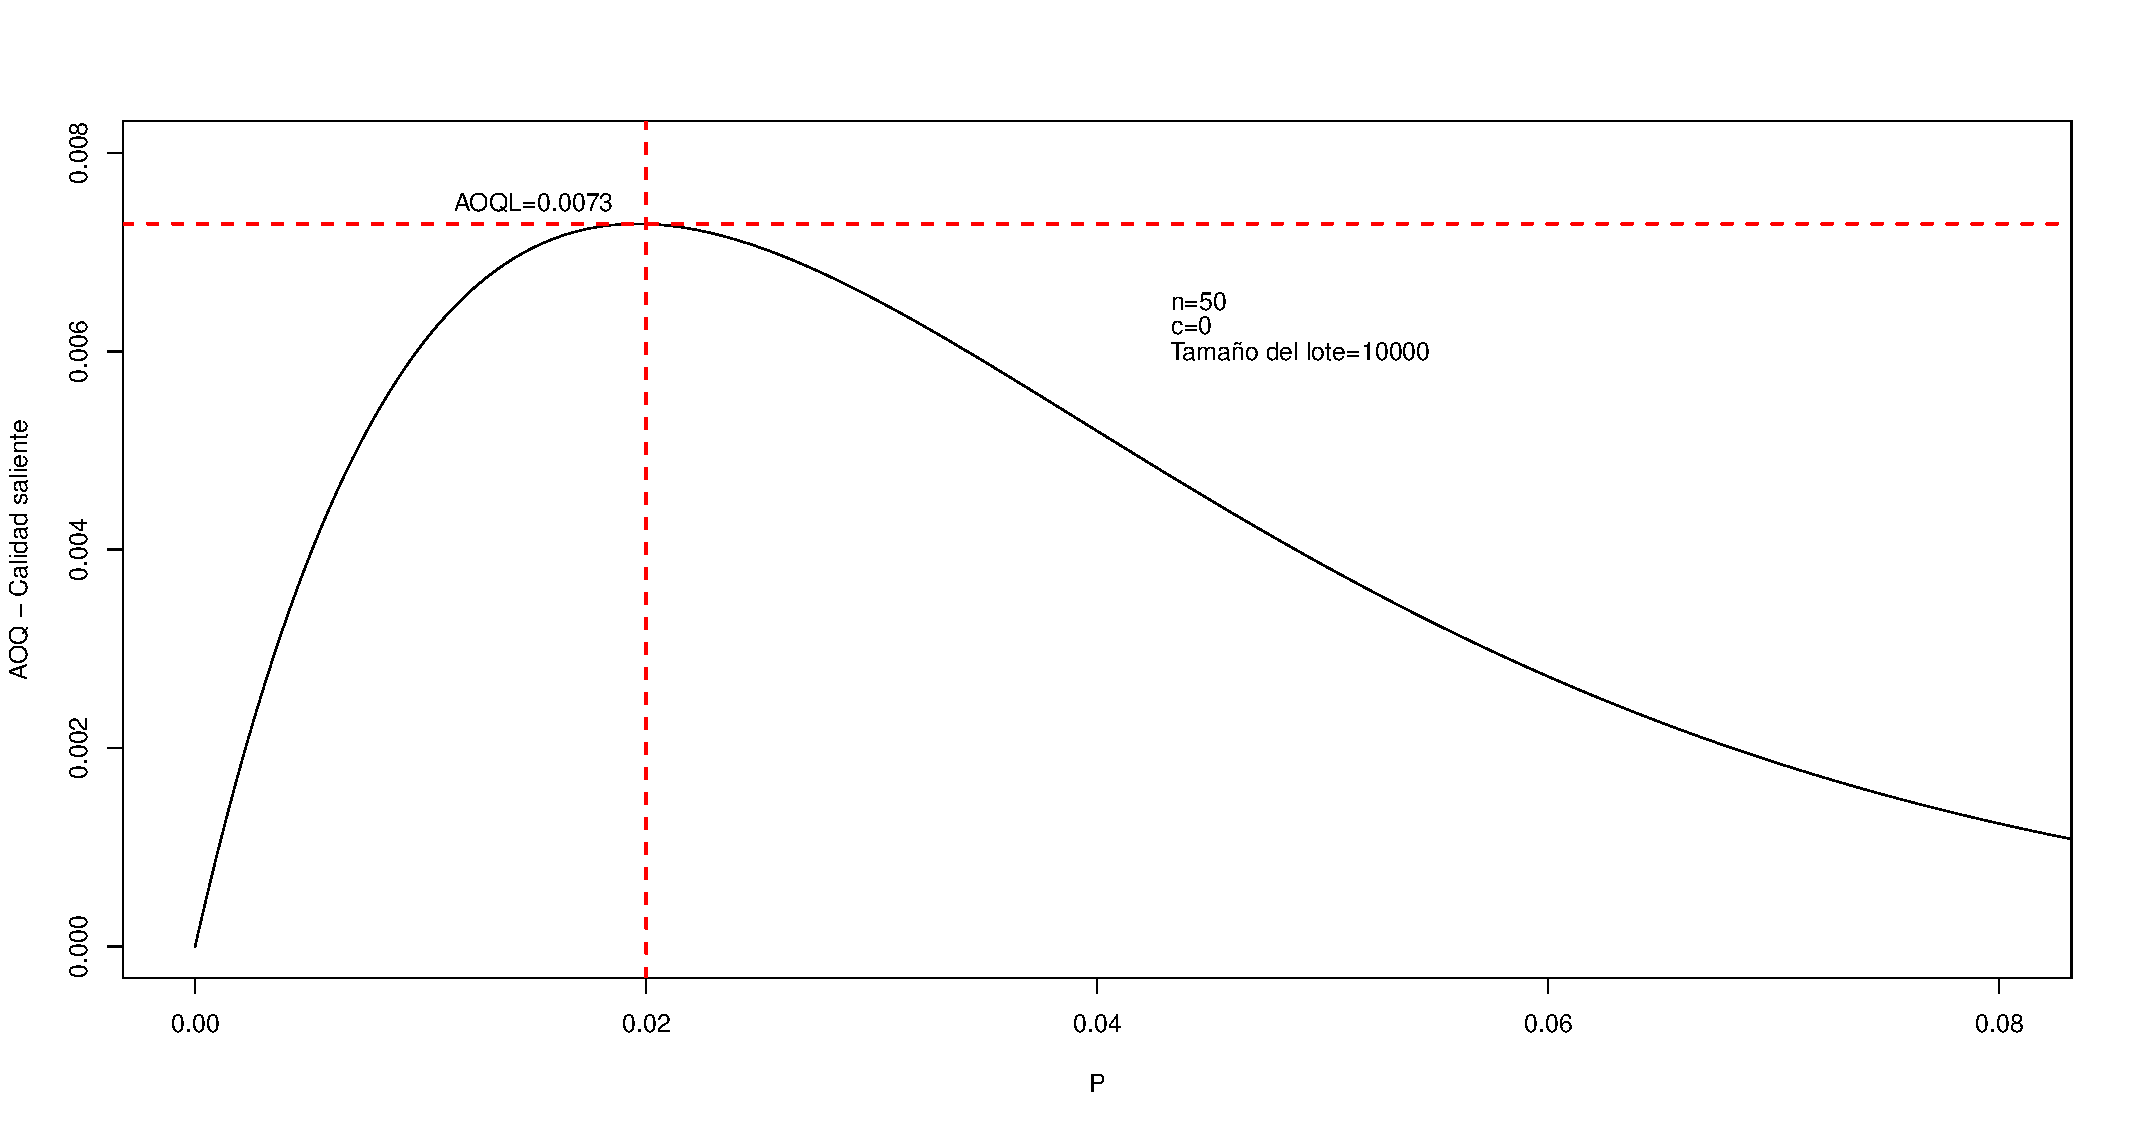
\includegraphics[scale=0.45]{IMAGENES/Figura2.pdf}
  \caption{Ejemplos curvas de operaci\'{o}n para lotes grandes $n/N<0.1$}
\end{figure}

~\\En el muestreo de aceptaci\'{o}n de lotes, se deben determinar ciertos par\'{a}metros que nos permitan decidir si rechazamos o aceptamos el lote a partir de los datos recogidos en la muestra, esos par\'{a}metros son:
\item N\'{u}mero de aceptaci\'{o}n: Es el n\'{u}mero de unidades infestadas o el n\'{u}mero de plagas individuales permitidas en una
muestra de determinado tama\~{n}o, antes de que se tomen medidas fitosanitarias.\cite{MUES}
\item Nivel de detecci\'{o}n:Es el porcentaje o la proporci\'{o}n de infestaci\'{o}n m\'{i}nimo que detectar\'{a} la metodolog\'{i}a de muestreo
al nivel de eficacia de detecci\'{o}n y el nivel de confianza especificado.\cite{MUES}
\item Nivel de confianza:Indica la probabilidad de que un env\'{i}o con un grado de infestaci\'{o}n que exceda el nivel de
detecci\'{o}n ser\'{a} detectado. Se suele utilizar un nivel de confianza del 95\%.\cite{MUES}
\item Eficacia de la detecci\'{o}n: La eficacia de la detecci\'{o}n es la probabilidad de que la inspecci\'{o}n o la prueba de diagn\'{o}stico de una o m\'{a}s unidades infestadas detectar\'{a} una plaga. En general, no deber\'{i}a suponerse que habr\'{a} un 100\% de eficacia.\cite{MUES}
\item Tama\~{n}o de la muestra: Es la cantidad de unidades seleccionadas del lote o env\'{i}o que se inspeccionar\'{a}n o someter\'{a}n a
pruebas de diagn\'{o}stico.\cite{MUES}
\item Nivel de tolerancia:Se refiere al porcentaje de infestaci\'{o}n de todo el env\'{i}o o lote que constituye el umbral para la acci\'{o}n fitosanitaria.En general, se utiliza un nivel de tolerancia 0.\cite{MUES}
\end{itemize}

\chapter{Metodolog\'{i}a}
~\\En esta secci\'{o}n se presenta la metodol\'{o}gica de la investigaci\'{o}n para dar soluci\'{o}n a la pregunta problema y a los objetivos planteados. Como primer punto analizamos las caracter\'{i}sticas que presentan las unidades muestrales teniendo en cuenta sus tipos y c\'{o}mo estas se encuentran distribuidas en los lugares de muestreo. Posterior a esto, como segundo punto se desarrollar\'{a}n diferentes propuestas muestrales que se podr\'{i}an implementar y se probar\'{a}n por medio de estudios de simulaci\'{o}n en distintos escenarios contextuales, tratando de abarcar todas las posibles situaciones que puedan ocurrir con el objetivo de evaluar cu\'{a}l de estas propuestas es la m\'{a}s \'{o}ptima. 

\section{Visita viveros}
Se visitaron dos viveros ubicados en Caicedonia - Valle del Cauca y en Calarc\'{a} - Quind\'{i}o, los cuales presentaban una capacidad m\'{a}xima aproximada de 70000 y 120000 plantas respectivamente. Se utiliz\'{o} una gu\'{i}a de observaci\'{o}n de elaboraci\'{o}n propia, la cual ayud\'{o} en el proceso de extraer la informaci\'{o}n necesaria para aplicar la metodolog\'{i}a y para el respectivo estudio de simulaci\'{o}n.

\section{Categorizaci\'{o}n de lotes} 

Para este punto se categorizar\'{a}n los lotes seg\'{u}n su tama\~{n}o con el fin de conocer qu\'{e} plan aplicar para cada tama\~{n}o del lote ($N$), esto es qu\'{e} tama\~{n}o de la muestra tomar cuando el lote es peque\~{n}o, mediano o grande; las categor\'{i}as se definir\'{a}n con rangos de tama\~{n}os.

\section{Dise\~{n}o del plan de muestreo en campo}

Para este punto se dise\~{a}ar\'{a}n las propuestas metodol\'{o}gicas que se implementar\'{a}n en los viveros con el fin de que la muestra recogida no solo sea aleatoria si no tambi\'{e}n representativa.

\section{Calculo de los tama\~{n}os de muestra para cada categor\'{i}a (Metodolog\'{i}a AoZ)} 

Se har\'{a} uso de la metodolog\'{i}a de los panes $c=0$ para calcular los tama\~{n}os de muestra correspondiente en cada categor\'{i}a previamente definida, esto con el fin de que cada rango de tama\~{n}o tenga un respectivo tama\~{n}o de muestra o porcentaje de plantas a muestrear.

\section{Calculo de los indicadores de desempe\~{n}o (AOQ, AOQL, ATI, OC)}

Una vez dise\~{n}ado el plan de muestreo y definido qu\'{e} tama\~{n}os de muestra se van a utilizar, pasamos a evaluar el dise\~{n}o muestreal, esto lo hacemos a partir de los indicadores del dise\~{n}o y sus respectivas curvas. Cada una nos dir\'{a} qu\'{e} tan bueno es el muestreo, qu\'{e} riesgos se llegan a correr en cuanto a la probabilidad de aceptar lotes con $x$ cantidad de plantas infectadas, tambi\'{e}n la calidad promedio de salida y la cantidad de plantas que se deber\'{i}an inspeccionar con dicho plan si existen $x$ cantidad de plantas infectadas en el lote.

\section{Categorizaci\'{o}n de los viveristas seg\'{u}n el nivel de riesgo} 

Luego de tener todo lo respectivo al muestreo, se planea crear 3 niveles de riesgo, flexible, normal y riguroso, esto para tener en cuenta en el muestreo el historial de los viveristas y ``premiar'' a los que mantengan una calidad en sus viveros alta, as\'{i} pues los viveristas comenzar\'{a}n en un nivel de riesgo normal, y pasaran a flexible o riguroso dependiendo de la cantidad de lotes ``buenos o malos'' que tengan en su historial, as\'{i} los que tengan una calidad ``buena'' en sus viveros tendr\'{a}n tama\~{n}os de muestra mas peque\~{n}os y por el contrario los que tengan calidad ``mala'' (varios lotes rechazados) pasaran a tener un  tama\~{n}o de muestra mayor, lo que implica m\'{a}s costos.

\section{Validaci\'{o}n de los planes por medio de simulaci\'{o}n}

Por \'{u}ltimo se validar\'{a}n los planes dise\~{n}ados utilizando herramientas computacionales donde, se simular\'{a}n todos los posibles escenarios de los viveros con los diferentes planes para as\'{i} conocer si estos cumplen con el objetivo de detectar lotes infectados con una confianza alta.



\chapter{Resultados}
\chapter{Cap\'{\i}tulo...}
Se deben incluir tantos cap\'{\i}tulos como se requieran; sin embargo, se recomienda que el Trabajo de Grado tenga un m\'{\i}nimo 3 cap\'{\i}tulos y m\'{a}ximo de 6 cap\'{\i}tulos (incluyendo las conclusiones).\\ 
\chapter{Conclusiones y recomendaciones}
\section{Conclusiones}
Las conclusiones constituyen un cap\'{\i}tulo independiente y presentan, en forma l\'{o}gica, los resultados del trabajo de grado. Las conclusiones deben ser la respuesta a los objetivos o prop\'{o}sitos planteados. Se deben titular con la palabra conclusiones en el mismo formato de los t\'{\i}tulos de los cap\'{\i}tulos anteriores (T\'{\i}tulos primer nivel), precedida por el numeral correspondiente (seg\'{u}n la presente plantilla).\\

\section{Recomendaciones}
Se presentan como una serie de aspectos que se podr\'{\i}an realizar en un futuro para emprender trabajos similares o fortalecer lo realizado. Deben contemplar las perspectivas del estudio, las cuales son sugerencias, proyecciones o alternativas que se presentan para modificar, cambiar o incidir sobre una situaci\'{o}n espec\'{\i}fica o una problem\'{a}tica encontrada. Pueden presentarse como un texto con caracter\'{\i}sticas argumentativas, resultado de una reflexi\'{o}n acerca del trabajo de grado.\\



\begin{appendix}
\chapter{Anexo: Nombrar el anexo A de acuerdo con su contenido}\label{AnexoA}
Los Anexos son documentos o elementos que complementan el cuerpo de la tesis o trabajo de investigaci\'{o}n y que se relacionan, directa o indirectamente, con el trabajo de grado, tales como acetatos, cd, normas, etc.\\

\chapter{Anexo: Nombrar el anexo B de acuerdo con su contenido}
A final del documento es opcional incluir \'{\i}ndices o glosarios. \'{E}stos son listas detalladas y especializadas de los t\'{e}rminos, nombres, autores, temas, etc., que aparecen en el mismo. Sirven para facilitar su localizaci\'{o}n en el texto. Los \'{\i}ndices pueden ser alfab\'{e}ticos, cronol\'{o}gicos, num\'{e}ricos, anal\'{\i}ticos, entre otros. Luego de cada palabra, t\'{e}rmino, etc., se pone coma y el n\'{u}mero de la p\'{a}gina donde aparece esta informaci\'{o}n.\\

\chapter{Anexo: Nombrar el anexo C de acuerdo con su contenido}
Manejo de la Bibliograf\'{\i}a: la bibliograf\'{\i}a es la relaci\'{o}n de las fuentes documentales consultadas por el investigador para sustentar sus trabajos. Su inclusi\'{o}n es obligatoria en todo trabajo de grado. Cada referencia bibliogr\'{a}fica se inicia contra el margen izquierdo.\\

La NTC 5613 establece los requisitos para la presentaci\'{o}n de referencias bibliogr\'{a}ficas citas y notas de pie de p\'{a}gina. Sin embargo, se tiene la libertad de usar cualquier norma bibliogr\'{a}fica de acuerdo con lo acostumbrado por cada disciplina del conocimiento. En esta medida es necesario que la norma seleccionada se aplique con rigurosidad.\\

Es necesario tener en cuenta que la norma ISO 690:1987 (en Espa\~{n}a, UNE 50-104-94) es el marco internacional que da las pautas m\'{\i}nimas para las citas bibliogr\'{a}ficas de documentos impresos y publicados. A continuaci\'{o}n se lista algunas instituciones que brindan par\'{a}metros para el manejo de las referencias bibliogr\'{a}ficas:\\

\begin{center}
\centering
\begin{tabular}{|p {7.5 cm}|p {7.5 cm}|}\hline
Instituci\'{o}n & Disciplina de aplicaci\'{o}n\\\hline
Modern Language Association (MLA)&Literatura, artes y humanidades\\\hline
American Psychological Association (APA)&Ambito de la salud (psicolog\'{\i}a, medicina) y en general en todas las ciencias sociales\\\hline
Universidad de Chicago/Turabian &Periodismo, historia y humanidades.\\\hline
AMA (Asociaci\'{o}n M\'{e}dica de los Estados Unidos)&Ambito de la salud (psicolog\'{\i}a, medicina)\\\hline
Vancouver &Todas las disciplinas\\\hline
Council of Science Editors (CSE)&En la actualidad abarca diversas ciencias\\\hline
National Library of Medicine (NLM) (Biblioteca Nacional de Medicina)&En el \'{a}mbito m\'{e}dico y, por extensi\'{o}n, en ciencias.\\\hline
Harvard System of Referencing Guide &Todas las disciplinas\\\hline
JabRef y KBibTeX &Todas las disciplinas\\\hline
\end{tabular}
\end{center}

Para incluir las referencias dentro del texto y realizar lista de la bibliograf\'{\i}a en la respectiva secci\'{o}n, puede utilizar las herramientas que Latex suministra.

\end{appendix}
\addcontentsline{toc}{chapter}{\numberline{}Bibliograf\'{\i}a}

\bibliographystyle{agsm}
\bibliography{BiblioPAE}
\end{document}
